% !TEX root = ../../main.tex

\section{Structural stability and the mechanics of non-linear materials}

\subsection{Column buckling and the normalised slenderness approach}

Perfect columns are idealised structural members that are perfectly straight and exhibit elastic--perfectly plastic behaviour. The strength of such a member is bounded by two limiting modes of failure: geometric instability and material yielding. The former is governed by the Euler critical buckling load, which for a pin-ended column is
%
\begin{equation}
    N_{\mathrm{cr}} = \frac{\pi^2 E I}{L^2},
    \label{eq:euler}
\end{equation}
%
where $E$ is Young's modulus, $I$ is the second moment of area and $L$ is the member length \parencite{timoshenko2009}. The latter is governed by the squash load $N_{\mathrm{y}} = A f_{\mathrm{y}}$, where $A$ is the cross-sectional area and $f_{\mathrm{y}}$ is the yield stress. Together these define the normalised slenderness $\lambdabar$, which collapses the column's geometry, material and length into a single dimensionless parameter, while the ultimate load $N_{\mathrm{u}}$ is normalised by the squash load to give the buckling reduction factor $\chi$:
%
\begin{equation}
    \lambdabar = \sqrt{\frac{N_{\mathrm{y}}}{N_{\mathrm{cr}}}},
    \qquad
    \chi = \frac{N_{\mathrm{u}}}{N_{\mathrm{y}}}.
    \label{eq:slenderness-chi}
\end{equation}
%
As illustrated in \cref{fig:chi-lambdabar-baseline}, the theoretical maximum strength of a perfect column forms a sharp $\chi$--$\lambdabar$ baseline: a pure squashing plateau ($\chi = 1$) for stocky columns and an elastic Euler hyperbola ($\chi = \lambdabar^{-2}$) for slender columns, the two regimes meeting at $\lambdabar = 1$ \parencite{trahair2008}.

\begin{figure}[tbp]
  \centering
  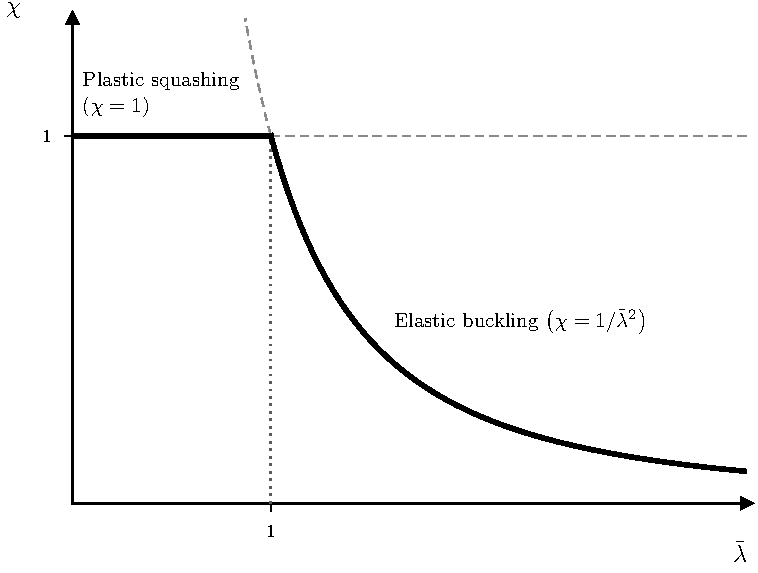
\includegraphics[width=0.75\textwidth]{figures/chi-lambdabar-baseline.pdf}
  \caption[Idealised column strength baseline]{%
    Buckling reduction factor $\chi$ against normalised slenderness $\lambdabar$
    for a perfect, elastic--perfectly plastic column: the lower envelope of the
    squash plateau ($\chi = 1$) and the Euler hyperbola ($\chi = \lambdabar^{-2}$),
    which meet at $\lambdabar = 1$.}
  \label{fig:chi-lambdabar-baseline}
\end{figure}

Real columns, however, never reach the perfect baseline because they carry imperfections such as initial crookedness, residual stresses, and load eccentricities. As a result, failure is observed below the theoretical bounds described, particularly at intermediate slenderness ($\lambdabar \approx 0.7\text{--}1.5$) where instability and yielding interact.




\begin{comment}

Paragraph 2 --> real columns fall below baseline
- State the gap (why do real columns fall below the baseline?)
- What are the consequences? = failure below both theoretical bounds --> greatest at intermediate slenderness (0.7 < λ < 1.5) where instability and yielding interact
- Classical analytical treatment --> Perry Robertson approach --> initally curved strut then yields a smooth strength curve that is below the baseline
- Imperfection knockdown is the basis of the modern design curves e.g. EC3

Paragraph 3 --> inelastic buckling of non-linear materials
1. Materials that yield gradually --> stiffness decreases before Ny is reached --> smooth transition between two regimes
2. Load at which buckling initiated is governed by the tangent modulus rather than initial elastic modulus
3. This makes the precise shape of the stress--strain curve imporant --> link to next section

Paragraph 4 --> bounding scope
1. global flexural buckling 
2. local buckling and torsional buckling out of scope
3. Give reason for exclusion

\subsection{The Ramberg--Osgood constitutive law for non-linear materials}
\label{sec:ramberg-osgood}

Paragraph 1 --> why stainless steel differs from carbon steel
1. carbon steel is conventionally idealised as linear-elastic, perfectly-plastic, with a sharp, well-defined yield point and a yield plateau.
2. stainless steel (and aluminium, and cold-formed steel) instead shows a rounded stress-strain response with no yield plateau and pronounced strain hardening — so there is no single physical yield stress.
3. in its place, an equivalent yield is defined conventionally as the 0.2$%$ proof stress, σ_0.2 — the stress at 0.2$%$ permanent strain.
4. (hook to figure): contrast the two responses visually.
5. Figure 2.2 — a stress-strain comparison showing the bilinear carbon-steel idealisation (sharp yield + plateau) against the rounded stainless curve, with the 0.2% offset construction marked. Introduce it here: "Figure 2.2 contrasts the two responses..." This is the one figure that genuinely earns its place in 2.1.2 — it makes "rounded vs. bilinear" immediate in a way prose can't.

Paragraph 2 — the Ramberg–Osgood law itself

Sentence 1: introduce the law as the standard three-parameter description of this rounded response.
Sentence 2: present the displayed, numbered equation (the ε = σ/E + 0.002(σ/σ_0.2)^n form), defining each symbol immediately after — E, σ_0.2, and the hardening exponent n.
Sentence 3: explain what n controls physically — it governs the sharpness of the knee, with high n approaching the bilinear limit and low n giving a more gradual, rounded transition.
Citation: Ramberg & Osgood (1943) at the equation — the non-negotiable primary source.
Figure: none (you may add a small inset or second panel to Figure 2.2 showing curves for varying n, but only if it doesn't crowd the figure — optional, lean toward not).

Paragraph 3 — modern refinements for stainless steel (short, 3 sentences)

Sentence 1: note that the original single-stage law loses accuracy beyond the proof stress, over-predicting stress at high strain.
Sentence 2: describe the two-stage remedy — the basic law up to σ_0.2, and a modified expression above it referenced to the proof-stress point — and that this is the form adopted in Eurocode material modelling.
Sentence 3: note these models are now well-established and calibrated against large experimental databases.
Citations: Mirambell & Real (2000) and Rasmussen (2003) for the two-stage model; Gardner & Nethercot (2004) for the compound variant; Arrayago et al. (2015) for the modern database calibration. Don't cite all four in one breath — Mirambell & Real plus Rasmussen at the two-stage sentence, Arrayago et al. at the database sentence.
Figure: none.

Paragraph 4 — non-invertibility and its consequence (the bridge into 2.2)

Sentence 1: state the key analytical property — the law is strain-explicit (strain as a function of stress) and cannot be algebraically inverted to a closed-form stress-from-strain expression.
Sentence 2: draw the consequence — this non-invertibility historically obstructed closed-form solutions to buckling problems in these materials.
Sentence 3 (the hook into 2.2): conclude that the field has therefore relied on one of two routes — empirically-calibrated design curves, or iterative numerical methods — each of which the following section examines, and each of which the anchor model later circumvents.
Citation: Abdella (2006) for non-invertibility.
Figure: none.

\end{comment}

\endinput